%==========================================================
% The OpenCms Synchronisation Management
%==========================================================
\section{The OpenCms Synchronisation Management}
\label{synchronisationmanagement}

\subsection{Manage the properties for OpenCms Synchronisation}
%============================================================================
The synchronisation requires some entries in the {\dir registry.xml}. To make it easier for you to manage these entries there is a management tool in the backoffice. Only administrators are allowed to manage the synchronisation properties.
(Figure~\ref{syncicon}).

\begin{figure}[hbt]
\begin{center}
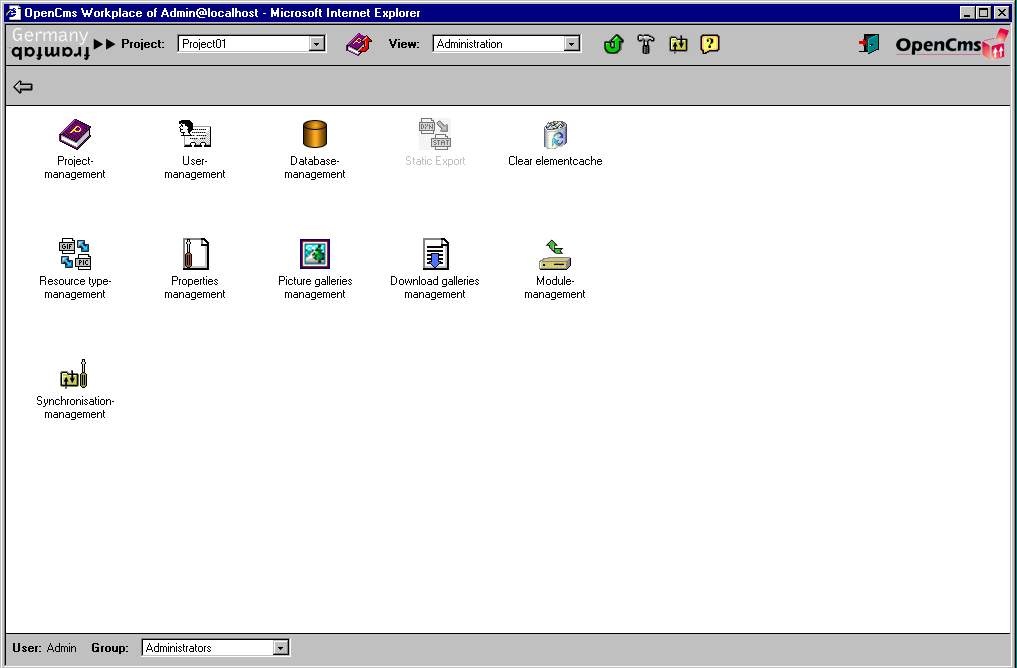
\includegraphics[width=\sgw]
                   {pics/synchronize/syncprop01.eps} 
\caption[The icon for synchronisation management]
           {The icon for synchronisation management}
\label{syncicon}
\end{center}
\end{figure} 

A click on the icon will open the dialog for synchronisation management.
If the entries for synchronisation already exist in the {\dir registry.xml}, they will be shown in the dialog.
(Figure~\ref{syncdialog}).

\begin{figure}[hbt]
\begin{center}
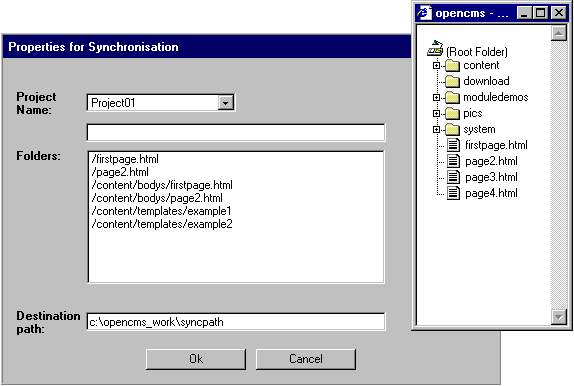
\includegraphics[width=\sgw]
                   {pics/synchronize/syncprop02.eps} 
\caption[The synchronisation management dialog]
           {The synchronisation management dialog}
\label{syncdialog}
\end{center}
\end{figure}

You can choose any project from the project list. The list contains your accessible projects accept the online project. So there must be at least one offline project. When you have chosen a project the folder tree, that you get with the folder button, shows the resources in this project. By clicking on a resource you can add it to the resource list for synchronisation.
You can also add resources by fill in the resource name into the field above the resource list and clicking the arrow button. To remove resources from the list you use the delete button.

The third entry that is needed is the destination path on your server.

When you choose all entries you can update the registry by clicking on 'OK'.
There will be errors if you left the project, the resource list or the destination path empty or if a resource can not be read from the choosen project.

%%% Local Variables: 
%%% mode: latex
%%% TeX-master: "OpenCmsDoc"
%%% End: